\begin{figure}[h]
	\begin{center}
		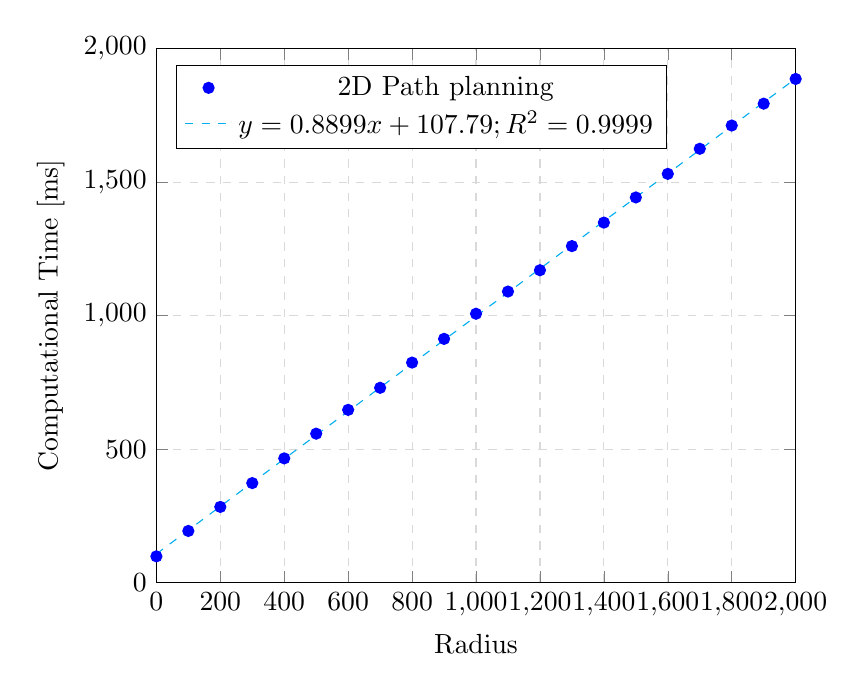
\begin{tikzpicture}
			\begin{axis}[
				width=0.8\linewidth, % Scale the plot to \linewidth
				grid=major, 
				grid style={dashed,gray!30},
				xlabel={Radius}, % Set the labels
				ylabel={Computational Time [ms]},
				legend pos=north west,
				xmin=0,
				xmax=2000,
				ymin=0,
				ymax=2000,
				]
				
				
				%2d test data
				\addplot[only marks, color=blue]
				table[row sep=crcr]{
					0 98.853165 \\
					100 193.98699\\
					200 283.95058\\
					300 373.10144\\
					400 465.5869\\
					500 558.11993\\
					600 647.20301\\
					700 729.78178\\
					800 824.24182\\
					900 912.9868\\
					1000 1007.04737\\
					1100 1090.12372\\
					1200 1169.9529\\
					1300 1260.2584\\
					1400 1348.2436\\
					1500 1442.4541\\
					1600 1530.6858\\
					1700 1624.6226\\
					1800 1711.6543\\
					1900 1793.4719\\
					2000 1885.9677\\
				}; 
				\addlegendentry{2D Path planning}
				
				%2d test regression
				\addplot[domain=0:2000, samples=100,no marks, color=cyan, style=dashed]
				{0.8899*x + 107.79};
				\addlegendentry{$y = 0.8899x + 107.79; R^2 =  0.9999$} 
			\end{axis}
		\end{tikzpicture}
		\caption{This plot illustrates the increase in computational time with increased collision detection, for the two-dimensional path-planning algorithm. Each point represents the average time needed to compute 100 paths, with equivalent parameters.}
		\label{plot:2dCollisionExp}
	\end{center}
\end{figure}